


%-------------------------------

\newpage

\section{Systematic Review and Modelography}{Revue Systématique et Modélographie}




\comment[JR]{la modélographie doit logiquement arriver après les études d'épistemo quanti, qui ont permis de donner un aperçu de l'horizon scientifique}



An ongoing work is the production of a synthesis of this overview, from a modular modeling point of view, combined with a purpose and scale classification. Already mentioned, modular modeling consists in the integration of heterogeneous processes and implementation of processes in order to extract the set of mechanisms giving the best fit to empirical data~\cite{cottineau2015incremental}. We can thus classify models described here according to their building bricks in terms of processes implemented and thus identify possible coupling potentialities. This work is a preliminary step for the analysis in quantitative epistemology developed in chapter~\ref{ch:quantepistemo}.



%%%%%%%%%%%%%%%%%%%%
\subsection[Systematic Review][Revue Systématique]{Systematic Review and Meta-analysis}{Revue systématique et Meta-analyse}


Tandis que les études menées précédemment proposaient de construire un horizon global de l'organisation des disciplines s'intéressant à notre question, nous proposons à présent une étude plus ciblée des caractéristiques de modèles existants. Nous proposons pour cela dans un premier temps une revue systématique, c'est à dire la construction d'un corpus répondant à certaines contraintes, suivie d'une meta-analyse, c'est à dire une tentative d'explication de certaines caractéristiques des modèles par des modèles statistiques.

\comment[JR]{également tenter une classif endogène des modèles : selon les caractéristiques récupérées.}











%%%%%%%%%%%%%%%%%%%%
\subsection{Modelography}{Modélographie}


Nous passons à présent à une analyse mixte inspirée par les résultats précédents, notamment pour la classification. Elle a pour but d'extraire et de décomposer précisément les ontologies, échelles et processus, puis d'étudier des liens possibles entre ces caractéristiques des modèles et le contexte dans lequel ils ont été introduits. Il s'agit ainsi de la meta-analyse en quelque sorte, que nous désignerons ici par modélographie.



%%%%%%%%%%%%%%%%%
\begin{figure}
\centering
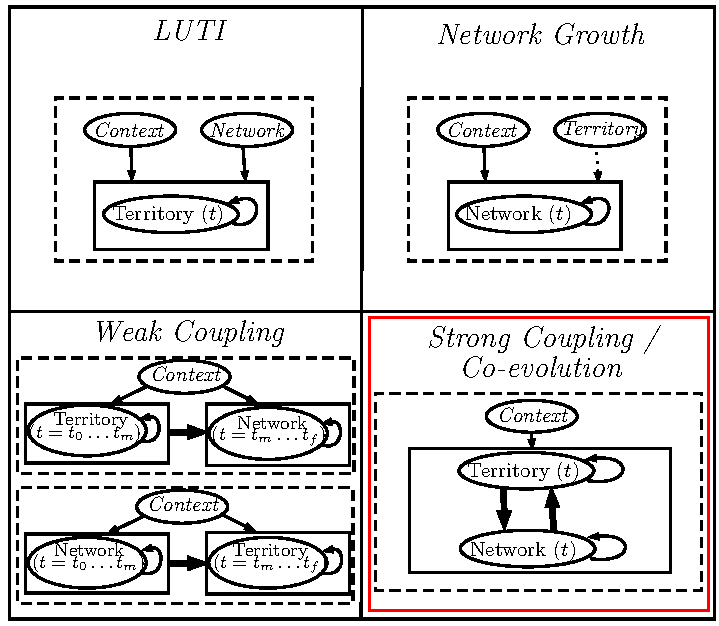
\includegraphics[width=\textwidth]{Figures/Modelography/coevolution}
\caption{}{Représentation schématique de la distinction entre différents types de modèles couplant territoires et réseaux.}
\end{figure}
%%%%%%%%%%%%%%%%%




caractéristiques : temporal and spatial span, scales, équilibre?, 


\todo{``bon choix'' de carac implique une bonne modularité de la classif obtenue dans une classif a priori (car on veut disciminer bien les modèles qu'on connait et qu'on juge différent) $\rightarrow$ faire une random forest regression et regarder structure endogène ; comparer à régressions simples.}









%%%%%%%%%%%%%%%%%%%%
\subsection{Discussion}{Discussion}

% préciser ici déjà des directions, clarifier question etc.












